%--------------------------------------------------------------------
% NENG 685 (intro to methods for neutral particle transport)

\documentclass[12pt]{article}
\usepackage[top=1in, bottom=1in, left=1in, right=1in]{geometry}
\usepackage[backend=biber]{biblatex}
\bibliography{te-de} 

\usepackage{setspace}
\onehalfspacing

\usepackage[hang,flushmargin]{footmisc} 
% 'hang' flushes the footnote marker to the left,  'flushmargin'  flushes the text as well.

\def\baselinestretch{1}
\setlength{\parindent}{0mm} \setlength{\parskip}{0.8em}

\newlength{\up}
\setlength{\up}{-4mm}

\newlength{\hup}
\setlength{\hup}{-2mm}

\usepackage{amssymb}
%% The amsthm package provides extended theorem environments
\usepackage{amsthm}
\usepackage{epsfig}
\usepackage{times}
\renewcommand{\ttdefault}{cmtt}
\usepackage{amsmath}
\usepackage{graphicx} % for graphics files

%% Draw figures yourself
\usepackage{tikz} 

% writing elements
\usepackage[version=4]{mhchem}

% The float package HAS to load before hyperref
\usepackage{float} % for psuedocode formatting
\usepackage{xspace}

% from Denovo Methods Manual
\usepackage{mathrsfs}
\usepackage[mathcal]{euscript}
\usepackage{color}
\usepackage{array}

\usepackage[pdftex]{hyperref}
\usepackage[parfill]{parskip}
\usepackage{cancel}

% math syntax
\newcommand{\nth}{n\ensuremath{^{\text{th}}} }
\newcommand{\ve}[1]{\ensuremath{\mathbf{#1}}}
\newcommand{\Macro}{\ensuremath{\Sigma}}
\newcommand{\rvec}{\ensuremath{\vec{r}}}
\newcommand{\omvec}{\ensuremath{\hat{\Omega}}}
\newcommand{\vOmega}{\ensuremath{\hat{\Omega}}}
%---------------------------------------------------------------------------
%---------------------------------------------------------------------------
\begin{document}
\begin{center}
{\bf NENG 685, Fall 17 \\
Introduction to Monte- Carlo\\
October 30, 2017}
\end{center}

\setlength{\unitlength}{1in}
\begin{picture}(6,.1) 
\put(0,0) {\line(1,0){6.25}}         
\end{picture}

%-------------------------------------------------------------

\section{Learning Objectives}

\begin{enumerate}
  \item Be able to define what a Monte-Carlo (MC) simulation is
  \item Be able to justify the choice of MC for radiation transport
  \item Be able to identify and explain the major components of MC radiation transport methods
  \item Provide examples of probabilistic representations of physics
  \item Distinguish between a PDF and CDF
  \item Distinguish between a discrete PDF (CDF) and continuous PDF (CDF)
  \item Describe the goal of random sampling
  \item Identify and implement the best random sampling technique for a given distribution
\end{enumerate}

%--------------------------------------------
%--------------------------------------------
%--------------------------------------------
\section*{What is Monte Carlo?}

Monte Carlo methods employ the use of random processes to determine a statistically-expected solution to a problem.  
These random processes can fulfill two roles:

\begin{itemize}
  \item Statistical approximation to mathematical equations
  \item Statistical approximations to physical processes
\end{itemize}

The basic concept for a MC simulation is to construct a random process for a problem and carry out a numerical simulation by N-fold sampling from a random number sequence.
These processes have been used extensively for hundreds of years to solve complicated problems of the time:

\begin{itemize}
  \item Comte du Buffon (1777): needle tossing experiment to calculate $\pi$
  \item Laplace (1786): random points in a rectangle to calculate $\pi$
  \item Lord Kelvin (1901): used random sampling to aid in evaluating time integrals associated with kinetic theory of gases
  \item Fermi (1930): was among the first to use random sampling methods to study neutron moderation while still in Rome, Italy
  \item 1947: Fermi, von Neumann, Frankel, Metropolis, Ulam, and others developed computer-oriented Monte Carlo method at Los Alamos to trace neutrons through fissionable materials; coined the term “Monte Carlo”
  \item Berger (1963): first complete coupled electron-photon transport code
\end{itemize}

MC is applicable to applications that are mathematically equivalent to \textit{integration over many dimensions.}
This can be useful when

\begin{itemize}
  \item Analytic integration is impossible
  \item Deterministic numerical integration is slow and/or requires error prone approximations.
\end{itemize}

The relatively straightforward approach of MC methods, combined with the fact that they easily simulation non-deterministic processes has led them to be used in a wide variety of fields:

\begin{itemize}
  \item High energy physics: many nucleon interactions
  \item Process engineering: Combine uncertainties in many variables
  \item Financial sector: Prices and rates of return for many objects (simulate many possible futures given trends and uncertainty)
  \item Risk analysis: Many individual probabilistic contributes to risk
\end{itemize}

However, MC methods often require significant computer time to general statistically significant results.
This can be overcome with parallel computing since MC methods are ``embarrassingly parralelizable".
Additionally, variance reduction (VR) methods have been developed that can be used to improve statistics with fewer particles. 
Finally, hybrid methods have been developed that use deterministic methods to accelerate MC calculations.
We will explore all of this over the next couple of lessons.

For now, let us explore the earliest use of MC to evaluate $\pi$ using the \href{08-02_Evaluating-Pi.ipynb}{iPython notebook}.

%--------------------------------------------
%--------------------------------------------
%--------------------------------------------
\section*{What is MC Radiation Transport?}

MC transport works by simulating many independent particles in a system.
For radiation transport, this works well as most of the physical processes that affect source generation and transport can be described as probabilistic events.  
The basic formulation of a MC transport method is to

\begin{itemize}
 \item Treat each physical process as a probabilistic process
 \item Randomly sample each process using an independent stream of random numbers
 \item Follow each particle from birth until it no longer matters
 \item Accumulate the contributions of each particle to find the statistically-expected mean behavior and variance
\end{itemize}

Unlike deterministic approaches, MC methods can readily model very complex things such as  pebble bed reactors.  Why?

\begin{figure}[h!]
\begin{center}
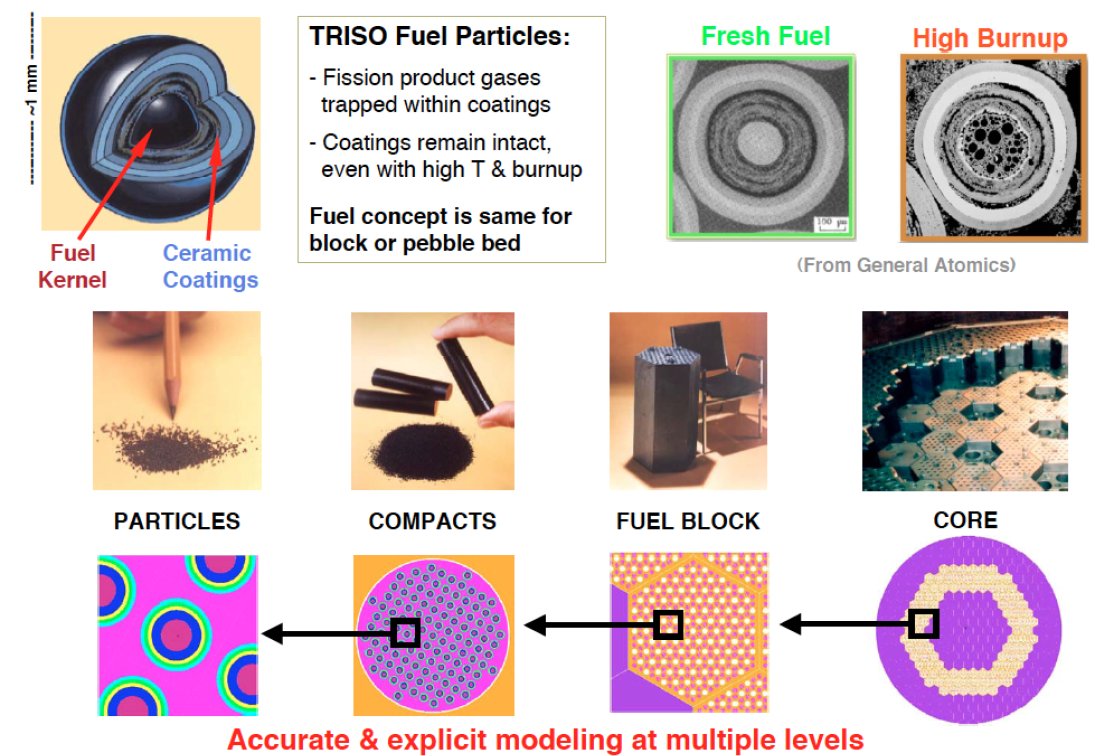
\includegraphics[scale=0.6]{../figs/triso.png}
\end{center}
\end{figure}

Is it worth considering

\begin{itemize}
  \item Is the independence assumption valid for all radiation transport?
  \item If not, where does the independence assumption cause problems?
  \item Are there radiation transport mechanisms that are deterministic instead of probabilistic?
\end{itemize}

%--------------------------------------------
\subsection*{Major Components of a MC Algorithm}

There are several common components of a MC algorithm that apply across any implementation considered:

\begin{itemize}
  \item PDFs: the physical/mathematical system must be described by a
set of pdfs.
  \item Random number generator: a source of random \#s uniformly
distributed on the unit interval.
  \item Sampling rule: prescription for sampling the pdf (given having
random \#s)
  \item Scoring: the outcomes must be accumulated/tallied for quantities
of interest
  \item Error estimation: an estimate of the statistical error (variance) of
the solution
  \item Variance Reduction: methods for reducing the variance and
computation time simultaneously
  \item Parallelization: efficient use of computers
\end{itemize}

For radiation transport, and example simple algorithm, using these components might be formulated as:

\begin{figure}[h!]
\begin{center}
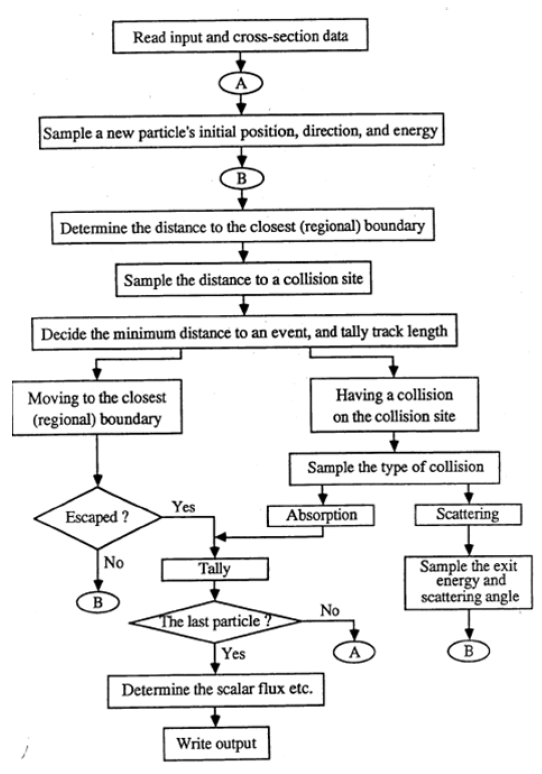
\includegraphics[scale=0.80]{../figs/mcAlgo.png}
\end{center}
\end{figure}


%--------------------------------------------
\subsection*{General Purpose MC Codes}

MC is the most common radiation transport method used across a wide range of applications.  
A non-inclusive list of common MC codes include:

\begin{itemize}
  \item MCNP: developed at LANL, distributed via RSICC, \url{http://rsicc.ornl.gov}
  \item Geant4: developed by a large collaboration in the HEP community, \url{http://geant4.web.cern.ch/geant4/}
  \item EGSnrc: developed at NRC (Canada), \url{http://www.irs.inms.nrc.ca/EGSnrc/EGSnrc.html}
  \item SERPENT: Developed by Dr. Jaakko Leppanen, VTT, Finland, \url{http://montecarlo.vtt.fi/}
  \item Shift: developed at ORNL, distributed via RSICC, \url{http://rsicc.ornl.gov}
  \item Mercury: developed at LLNL, \url{https://wci.llnl.gov/simulation/computer-codes/mercury}
\end{itemize}

%--------------------------------------------
%--------------------------------------------
%--------------------------------------------
\section*{Physics as Probability}

Various radiation related physical phenomena can be represented by probability distributions:

\begin{itemize}
  \item Photon emission energy: Each possible energy has a different probability (intensity)
  \item Scattering cross-sections: Each possible scattering angle has a different probability as a function of the energy
  \item Transmission through a medium: Probability of reaching a particular position depends on the cross-section
  \item Radioactive decay: Each decay event is probabilistic based on probability of individual atoms to tunnel through energy barriers
\end{itemize}

To implement MC, we must quantify the underlying probability distributions for the outcome of each physical event. 
We can then estimate the statistical moments of these distributions to get our physical answers.
Let's start by exploring probability density functions (PDFs) is more detail.


%--------------------------------------------
\subsection*{PDFs and CDFs}

In the MC simulation, all variables, $x$, have a Probability Density Function (PDF), $p(x)$, with the following characteristics:

\textbf{\underline{Continuous:}}
\begin{align*}
  p\{a \le x \le b\} &= \int_a^b \: p(x)dx \\
  p(x) &\ge 0 \\
  \int_{-\infty}^{\infty} \: p(x)dx &=1
\end{align*}

\textbf{\underline{Discrete:}}
\begin{align*}
  p(x = x_k) &= p_k \equiv p(x_k) \\
  k &= 1, \dots, N \\
  p_k &\ge 0 \\
  \sum_{k=1}^N &= 1
\end{align*}

The PDF represents the \textit{collective behavior} of the system.  
All PDFs, $p(x)$, have an associated Cumulative Distribution Function (CDF), $P(x)$, with the following properties:

\textbf{\underline{Continuous:}}
\begin{align*}
  p\left\lbrace x' \leq x \right\rbrace &= P(x) = \int_{-\infty}^x p(x')dx'\\
  & \\
  P(-\infty) &= 0 \:,\quad P(\infty) = 1 \\
  0 &\leq P(x) \leq 1 \\
  &\frac{dP(x)}{dx} \geq 0
\end{align*}

\textbf{\underline{Discrete:}}
\begin{align*}
  pP\left\lbrace x' \leq x \right\rbrace &= P_k \equiv P(x_k) = \sum_{j=1}^k p_j\\
  k &= 1, \dots, N \\
  P_0 &= 0 \:,\quad P_N = 1 \\
  0 &\leq P_k \leq 1 \\
  P_k & \geq P_{k-1} \\
\end{align*}

To demonstrate, consider a uniform probability distribution:

\begin{figure}[h!]
\begin{center}
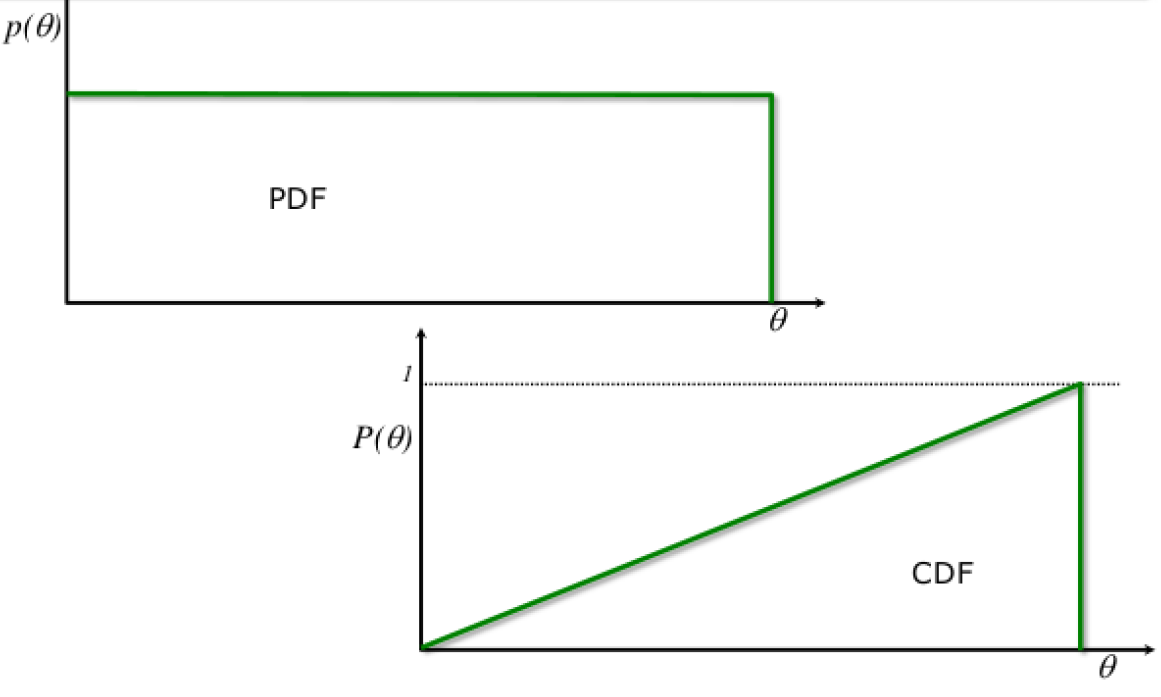
\includegraphics[scale=0.55]{../figs/pdf-cdf.png}
\end{center}
\end{figure}

Or a discrete probability distribution:

\begin{figure}[h!]
\begin{center}
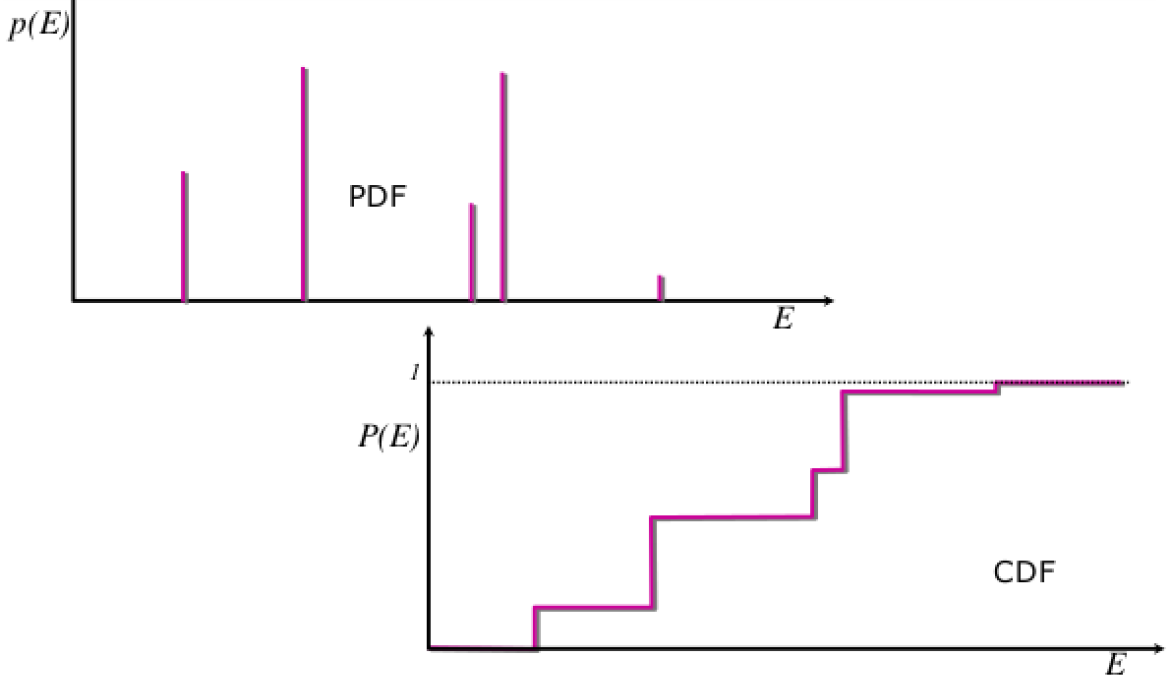
\includegraphics[scale=0.55]{../figs/discretePDF-CDF.png}
\end{center}
\end{figure}


%--------------------------------------------
\subsection*{Sampling Techniques}

Random sampling uses \underline{uniformly distributed random variables} to choose a value for a variable according to its PDF.  
The implementations can vary based on the form of the data and the physics process being modeled.
Some sampling techniques are

\begin{itemize}
  \item \textit{Basic} sampling techniques
  \begin{itemize}
    \item Direct discrete sampling
    \item Continuous discrete sampling
    \item Rejection sampling
  \end{itemize}
  
  \item \textit{Advanced }sampling techniques
  \begin{itemize}
    \item Histogram
    \item Piecewise linear
    \item Alias sampling
    \item Advanced continuous PDFs
  \end{itemize}
\end{itemize}

Several of these will be explored in the \href{08-03_Sampling.ipynb}{Sampling iPython notebook}

\end{document}
